\section{Silicon Tungsten SiD ECAL}\label{sec:Calorimeter:SiliconTungstenSiD}
Most recent update: 2015-06-15 \\
Contact person: Marty Breidenbach (email: mib@slac.stanford.edu)
\begin{figure}
	\centering
	\begin{minipage}[b]{.49\textwidth}
		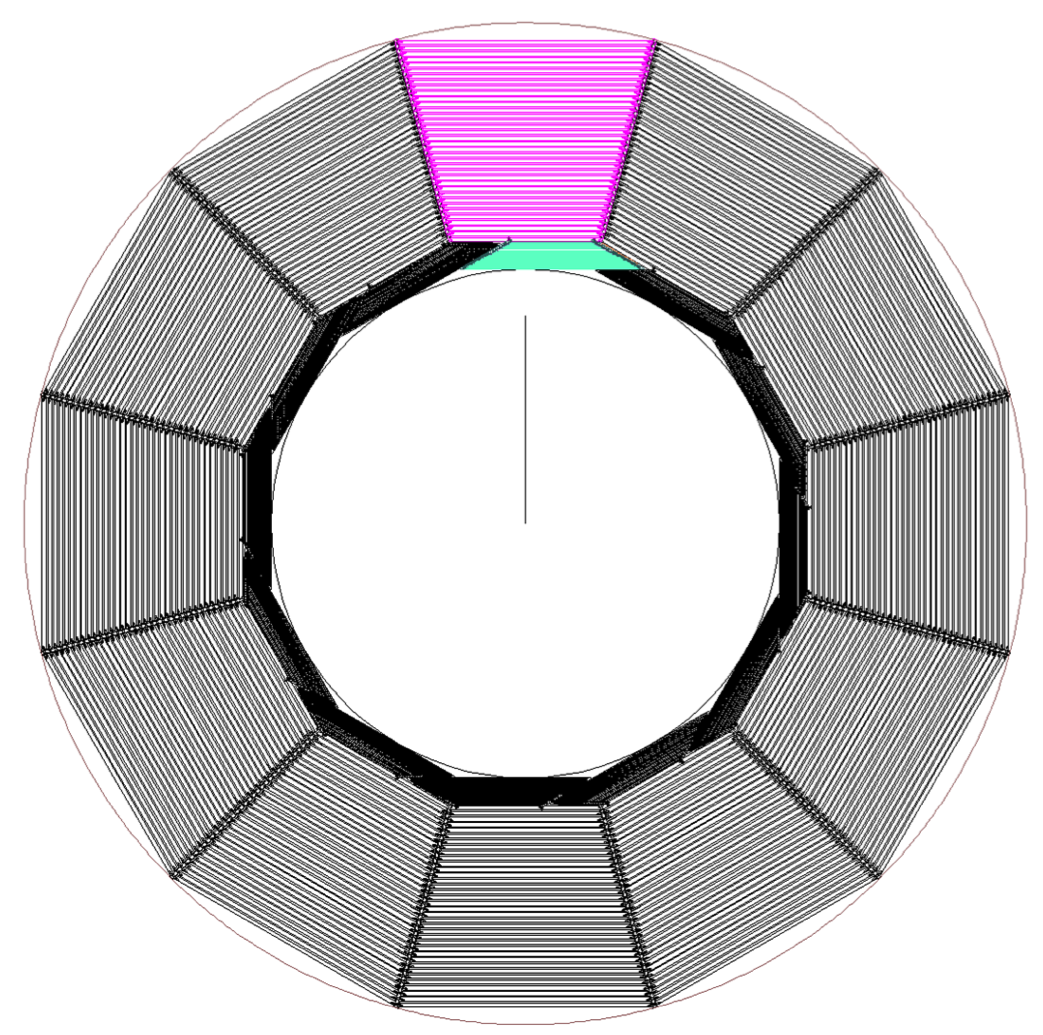
\includegraphics[width=\linewidth]{Calorimeter/SiliconTungstenSiD/cross_section}
		\caption{Outer HCAl and inner ECal barrel}
		\label{fig:Calorimeter:SiDECAL:crosssection}
	\end{minipage}\hfill
	\begin{minipage}[b]{.49\textwidth}
		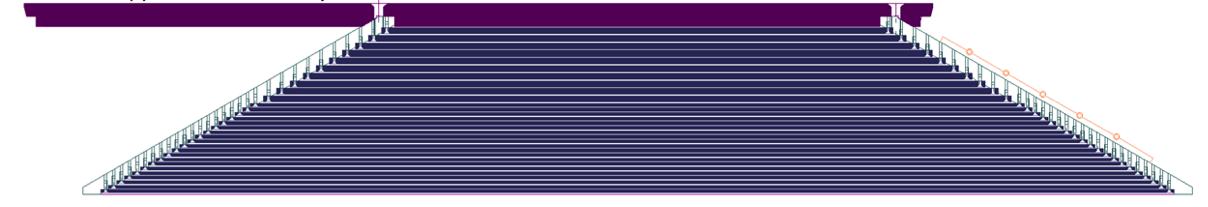
\includegraphics[width=\linewidth]{Calorimeter/SiliconTungstenSiD/ecalModule}
		\caption{ECal module}
		\label{fig:Calorimeter:SiDECAL:ecalModule}
	\end{minipage}
\end{figure}
\begin{figure}
	\begin{minipage}[b]{.29\textwidth}
		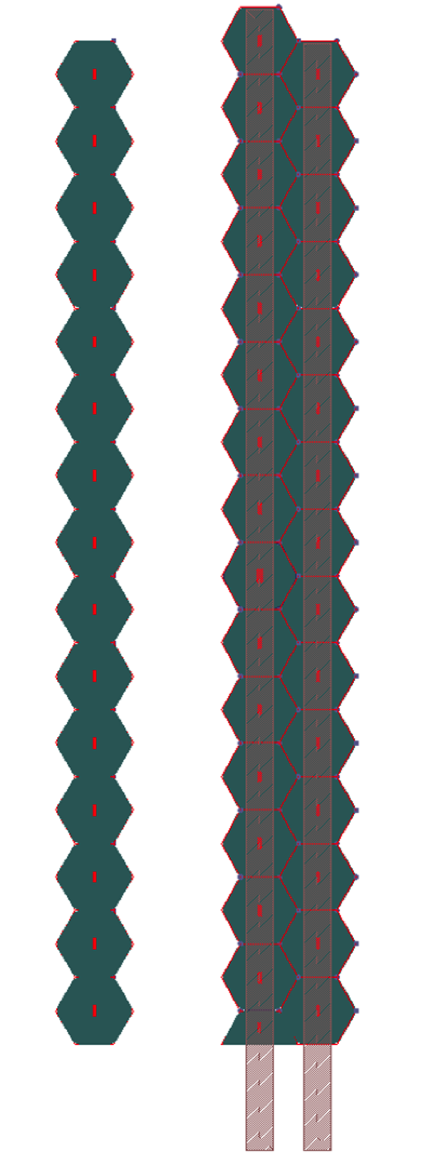
\includegraphics[width=\linewidth]{Calorimeter/SiliconTungstenSiD/hexagon}
		\caption{Hexagonal silicon detectors with flexible circuit interconnects}
		\label{fig:Calorimeter:SiDECAL:hexagon}
	\end{minipage}\hfill
	\begin{minipage}[b]{.65\textwidth}
		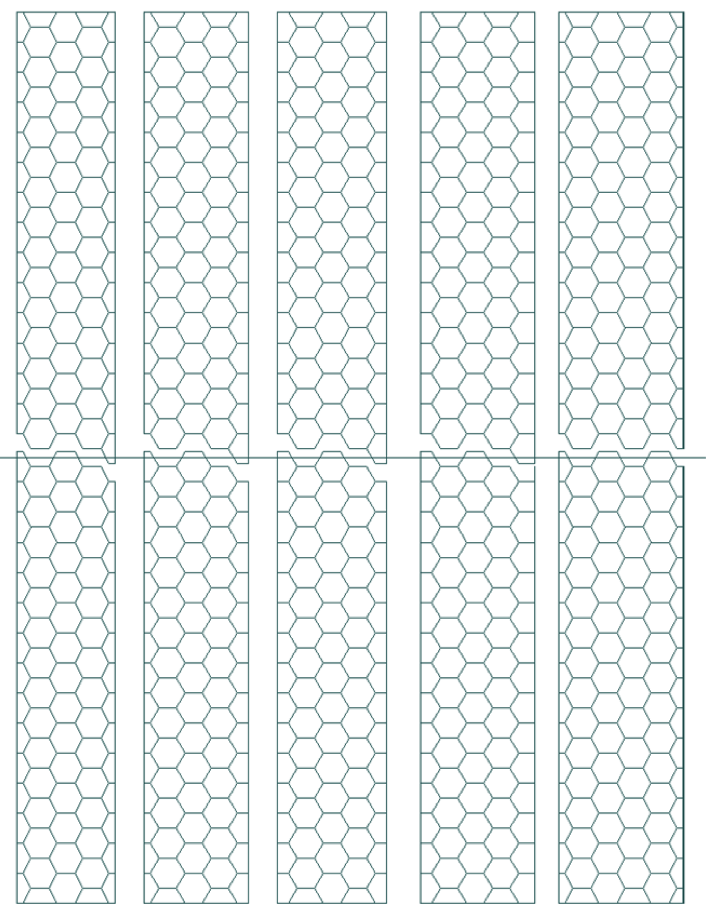
\includegraphics[width=\linewidth]{Calorimeter/SiliconTungstenSiD/siliconLayout}
		\caption{Silicon layout for five outer layers}
		\label{fig:Calorimeter:SiDECAL:siliconLayout}
	\end{minipage}
\end{figure}
\begin{figure}
	\begin{minipage}[b]{.49\textwidth}
		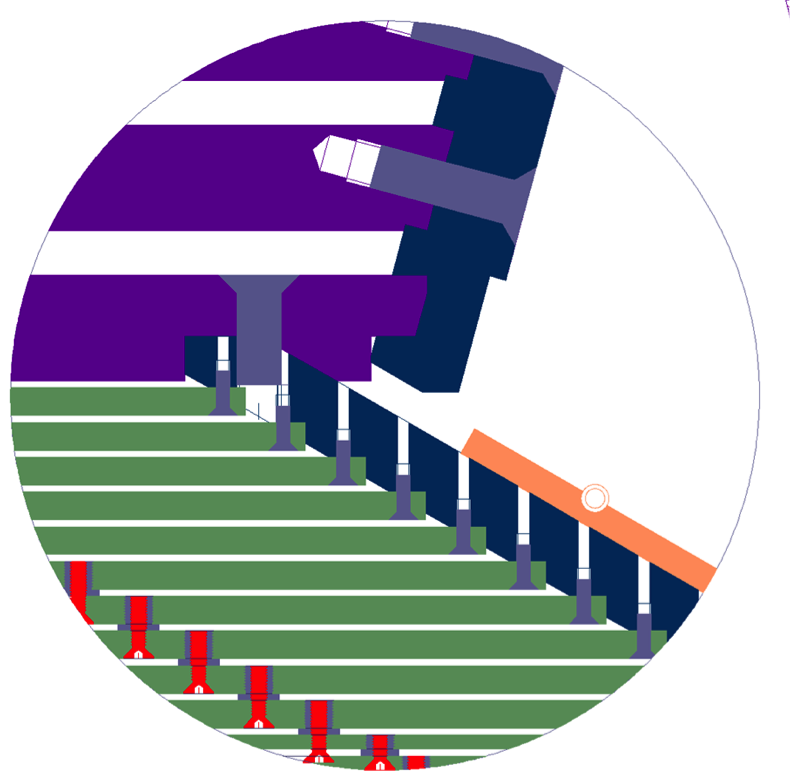
\includegraphics[width=\linewidth]{Calorimeter/SiliconTungstenSiD/edgeFasteners}
		\caption{Edge and field fasteners}
		\label{fig:Calorimeter:SiDECAL:edgeFasteners}
	\end{minipage}\hfill
	\begin{minipage}[b]{.49\textwidth}
		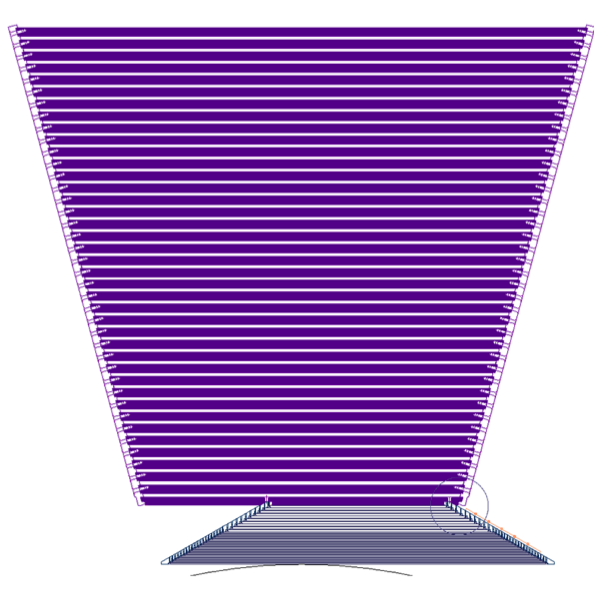
\includegraphics[width=\linewidth]{Calorimeter/SiliconTungstenSiD/ecalMounting}
		\caption{ECal to HCal mounting}
		\label{fig:Calorimeter:SiDECAL:ecalMounting}
	\end{minipage}
\end{figure}
\begin{figure}
	\begin{minipage}[b]{.49\textwidth}
		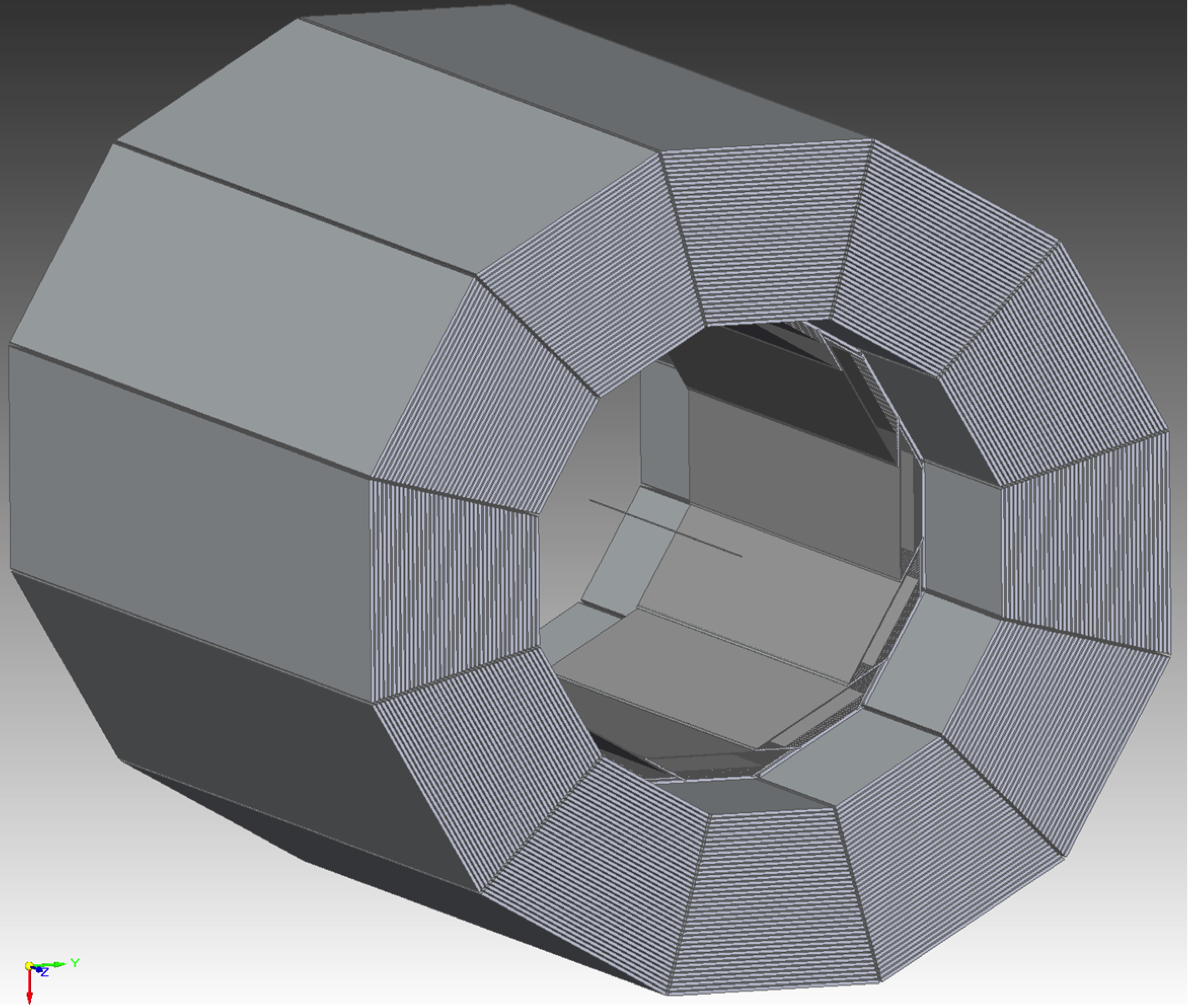
\includegraphics[width=\linewidth]{Calorimeter/SiliconTungstenSiD/HCalECal}
		\caption{HCal with integral ECal detector}
		\label{fig:Calorimeter:SiDECAL:HCalECal}
	\end{minipage}\hfill
	\begin{minipage}[b]{.49\textwidth}
		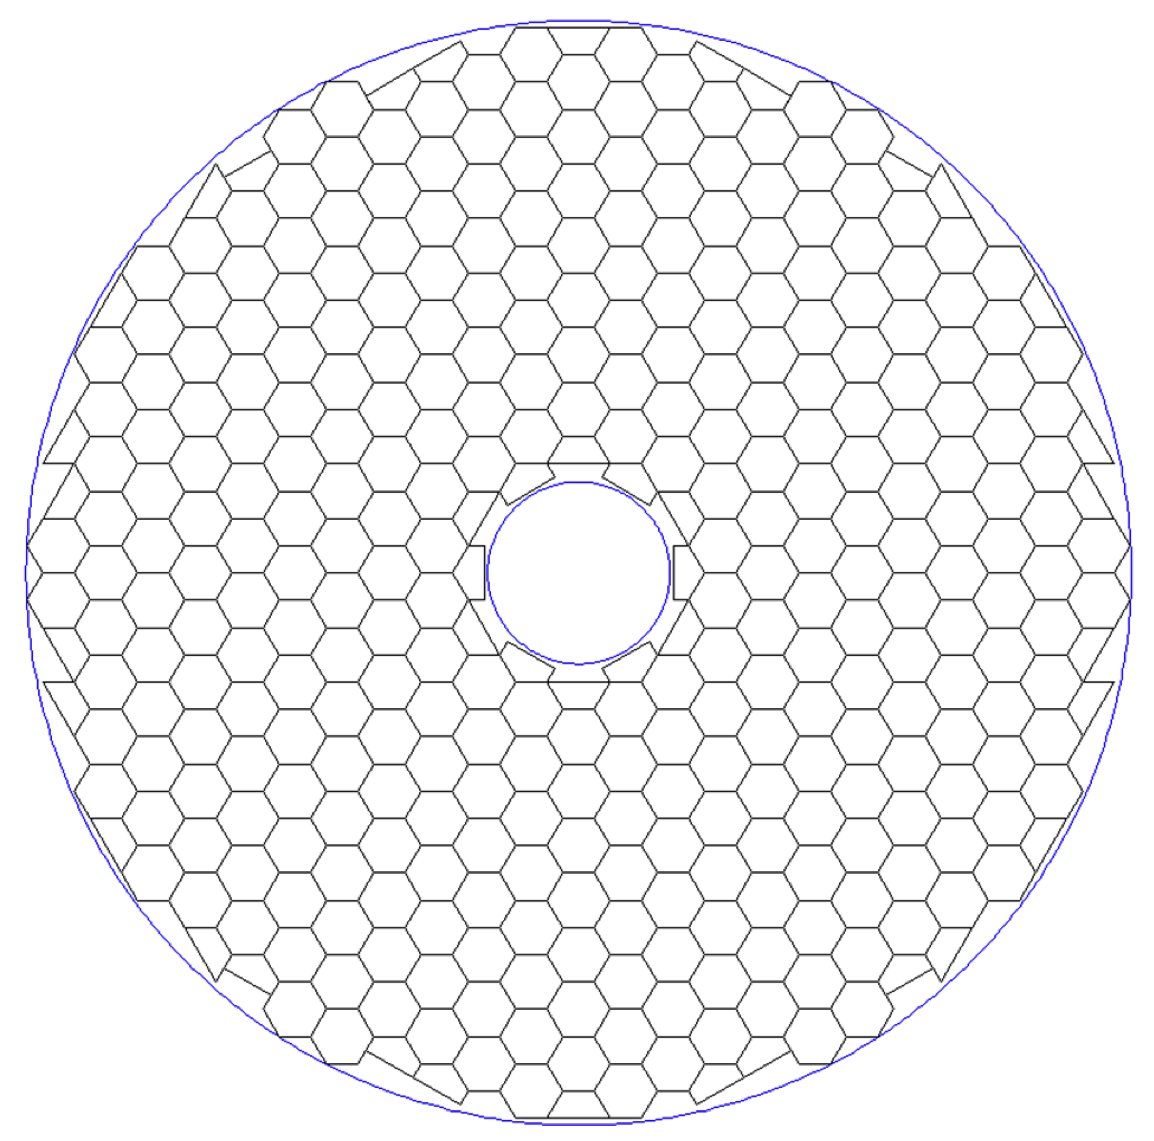
\includegraphics[width=\linewidth]{Calorimeter/SiliconTungstenSiD/endcapLayout}
		\caption{Endcap detector layout}
		\label{fig:Calorimeter:SiDECAL:endcapLayout}
	\end{minipage}
\end{figure}

This note describes the theory of the mechanical aspects of the E-Cal system for
SiD. The E-Cal barrel consists of stacks of tungsten heavy metal plates which
are arranged in modules surrounding the beamline. Full cylindrical coverage of
the baseline design is attained with twelve modules (see Figure~\ref{fig:Calorimeter:SiDECAL:crosssection}) occupying a
radial envelope from \SI{1265}{mm} to \SI{1409}{mm}. The total barrel length is \SI{3.53}{m}. Each
module uses 20 inner plates which are \SI{2.5}{mm} thick followed by ten \SI{5}{mm} thick
plates. Gaps between adjacent plates are \SI{1.25}{mm} and house the silicon detectors
with their associated cables (see Figure~\ref{fig:Calorimeter:SiDECAL:ecalModule}). These hexagonal silicon detectors
are electrically connected to each other with thin, flexible circuits which are
read out on both ends of a module (see Figure~\ref{fig:Calorimeter:SiDECAL:hexagon}). Panels of detectors increase
in width as they get closer to the beamline. To minimize silicon waste and to
maximize coverage, fractions of hexagons complete the panel edges (see Figure~\ref{fig:Calorimeter:SiDECAL:siliconLayout}). By cutting the silicon in strategic locations, only a few different silicon
shapes may be needed to achieve the 31 different panel widths. The tungsten
plates are connected together on their longitudinal edges as well as in the
field of detectors. Space for fasteners in the field is achieved by chamfering
the corners of the hexagonal detectors. The field fasteners hold the plates
together, provide a uniform \SI{1.25}{mm} standoff height, and assist with inter-plate
shear. The fasteners near the edges of the plates close the module profile and
lend torsional rigidity to the structure. An FEA simulation of the proposed
configuration should be done to properly size the fasteners (see Figure~\ref{fig:Calorimeter:SiDECAL:edgeFasteners}).The
modules, which weigh about 5 tons each, are mounted to stainless plates which
are used as the first layer of the next detector system (H-Cal). This first
H-Cal plate is unique in that its two longitudinal edges form a guide system to
locate the E-Cal to the H-Cal system. The H-Cal modules are first bolted
together to form the H-Cal barrel. Interleaving structural side battens maintain
spacing for the H-Cal plates and extend inward to the E-Cal support plates. The
inner ends of these battens act in concert as the female portion of the E-Cal
guide system. The E-Cal modules are slid into place in the inner H-Cal bore.
Extension plates complete the inner H-Cal first layer, since the E-Cal barrel is
shorter. H-Cal detector panels are installed after this structure is complete
(see Figure~\ref{fig:Calorimeter:SiDECAL:HCalECal}). Only simple detector layouts have been done for the E-Cal
endcaps so far. These layouts show that using full and partial hexagons could
yield fairly good coverage with only a few shapes. (see Figure~\ref{fig:Calorimeter:SiDECAL:endcapLayout}).

% \subsection{Participating Institutes}
% SLAC National Accelerator laboratory
% University of California, Davis
% University of California, Santa Cruz
% University of Oregon
% University of New Mexico

\subsection{Introduction}
KPiX is a 1,024 channel ``System on a Chip'' intended for bump bonding to large area Si sensors, enabling low multiple scattering Si strip tracking and high density Particle Flow calorimetry for SiD at the International Linear Collider (ILC).

Each channel consists of a dynamically switchable gain charge amplifier; shaping; threshold discrimination; and 4 sample and hold capacitors and 4 timing registers. The chip permits 4 separate measurements of amplitude and time of threshold crossing during each train, and amplitude digitization and readout during the intertrain period. The dynamic range is from sub minimum ionizing particle (mip) (\SI{320}{\micro\meter} silicon) to more than 2,000 mip. KPiX also has a calibration system for each channel, servos for leakage compensation, ``DC'' reset for asynchronous operation for testing with cosmic rays, and polarity inversion for use with GEMs and similar detectors. The noise floor is about \SI{0.15}{fC} ($\approx 1,000$ electrons), and the maximum signal is \SI{10}{pC} (utilizing the dynamic range switching). The full dynamic range corresponds to 17 bits.

\subsection{Recent Milestones}
ILC related R\&D in the US is largely unfunded and small efforts are being kept alive on the margins. The KPiX R\&D is such an example of necessary work for SiD that is marginally alive.
At this time, KPiX is seen as the baseline readout system for the tracker and electromagnetic calorimeter .  A stack of 13 EMCal sensors with bump bonded KPiX was assembled for a beam test at SLAC in the summer of 2013. That test discovered that two kinds of crosstalk are significant:
\begin{itemize}
	\item In-time crosstalk occurs due to parasitic coupling of traces on metal 2 of the sensor to other pixels. The level of crosstalk increases with the size of the signal, and decreases with increased speed of the front end charge amplifier (meaning increased current and power dissipation).  A new sensor design is being developed that uses metal 1 to shield the traces of metal 2, and these ideas will be tested in the next sensor prototype.
	\item Out-of-time cross talk occurs when many pixels are hit and reset simultaneously. The resets collectively cause other pixels to trigger, and a cascade builds up. This uses up all the KPiX buffers. The root cause of the problem appears to be some internal logic within KPiX that is not current limited, and will require design modification.
\end{itemize}
A more general issue is that both the EMCal and tracker sensors from Hamamatsu were ordered with Al pads, as it was believed that plating (by the zincate process) a stack of metals culminating with Au would be straightforward. This turns out to be wrong. After many attempts at University of California Davis (UCD) and local industry, IZM  has Ar ion etched the pad surfaces and sputtered a base layer, permitting the buildup of a stack that ended with Au, and permitting the attachment with solder bumps that had been placed during KPiX manufacture by TSMC. Testing of these sensors revealed $\approx 10\%$ pixel to pixel shorts and some opens of signal traces, that are suspected to be damage caused by the Ar ion etch. A new round of sensors has been ordered with the Metal 1 layer used to shield the Metal 2 traces from the diodes that they cross on the way to the KPiX bump pads, and with the Au pads being built by Hamamatsu.

An additional issue is that the Tracker sensor was planned to be wire bonded to its (very thin) cable. The sensor oxide layer is not strong enough to allow wire bonding without damage, and so must be solder bumped. The pad pitch is small, and solder bumping the cable will be challenging. The trouble with the wire bonding to the sensor was unexpected. Recent attempts with both bump bonding a cable and utilizing electrically conductive epoxy have failed. The best explanation is that the \SI{150}{\degreeCelsius} thermal cycles associated with these attachments increased the stress on the KPiX bonds and caused the sensor pads to separate from the sensor. It is belived that something went wrong with the Hamamatsu process on both types of sensors, and is related to the wire bonding problem.

Another concern is that the current design of KPiX has deadtime after a pixel has accepted a trigger. Only the triggered pixel is affected; all the other pixels are available for signals. This deadtime is different from the usual notion of data acquisition deadtime where the entire detector is unavailable, but the correction to the luminosity integral is easy. Finally, the buffer requirement (4 in the current version of KPiX) is being re-evaluated in SiD simulations. A possible new architecture for KPiX is in early stages of evaluation. Another approach is the development of Monolithic Active Pixel (MAP) sensors for both SiD sensors using thinned HVCMOS. The sensors would be approximately the same size as the current sensors. The tracker would have $40 \times \SI{500}{\micro\meter}$ pixels, and would only need one buffer. A prototype to evaluate the pixel performance is being designed now. The EMCal sensor will have $1 \times \SI{1}{mm}$ pixels which should limit the required dynamic range and eliminate range switching, but would still need 16 buffers.

A small mechanical engineering effort has started to study the structure of the EMCal. The Sid EMCal has emphasized thin gaps between the tungsten layers to minimize the Moliere radius, and this implies that the structure is connected by columns at the vertices of the sensors. This work has been carried out to the level of a pre-conceptual design.

\subsection{Engineering Challenges}
\subsection{Future Plans}
Assuming positive developments with Japan are announced soon, we expect the financial support to improve. It should be noted that an important effect of the withdrawal of support is that most of the US collaborators have been forced to move to other work.
\begin{itemize}
	\item EMCal Sensors: A second round of prototypes will be designed and ordered with rectangular layout; shielded traces, and Au pads.
	\item Tracker Sensors: The current prototypes will be evaluated, and if appropriate tested in a beam.
	\item KPiX: A new architecture with little (or no) deadtime will be evaluated. A decision will be made to develop this new architecture or incrementally improve the existing design.
	\item The EMCal mechanical structure will be pushed towards a conceptual design.
\end{itemize}
